


%\vspace{-5pt}
\subsection{The canonical and disease model parametrizations}

We provide two methods of specifying the alternative hypothesis in power analysis.
In addition to the familiar option of specification through disease models, we provide users with the option to perform power analysis via the canonical parameters, whose estimates are curated and readily available in the NHGRI-EBI GWAS Catalog:
\begin{itemize}
    \item Conditional distribution of risk allele variant among controls, i.e., risk allele frequency (RAF) in the Control group, denoted as $f$.
    \item Odds ratio (OR) of allele variants, denoted as $\text{R}$.
\end{itemize}
The canonical parameters ($f$ and $R$) are common to models of qualitative traits and invariant to model choices. 
This disease model-invariance allows users to perform power analysis valid for studies employing different models.
We also elucidate on the link between the two approaches, and provide a ``disease model converter'' in the application, performing explicit conversions from the disease models to the canonical parametrizations.

% From a statistical perspective, the disease model serves no role except to specify the distribution of the counts under the alternative.
% Here, statistical power is calculated directly based the quartet $(n_1, n_2, f, R)$, allowing us to perform power analysis valid for studies employing different models.

% We make the important distinction between RAF in the Control group ($f$), versus RAF among all subjects in the study, and RAF in the general population.
% Throughout this work and the software, RAF refers to the risk allele frequency in the Control group, consistent with the reporting standard of the NHGRI-EBI GWAS Catalog.

\vspace{-5pt}
\subsection{A test-independent power analysis}

While power calculations are necessarily tied to the statistical tests used, for many common association tests, statistical powers are asymptotically equivalent.
% For example, it is known that for tests of associations in contingency tables, the likelihood ratio (LR) test and Pearson's chi-square test enjoy the same power asymptotically.
% We further show that tests including, e.g., Welch's t-test (though not the student t-test) and LR tests for logistic regressions, also have asymptotically the same power, as long as the canonical parameters assume the same values. 
We show in the Supplement that the likelihood ratio test, chi-square test, Welch's t-test, and LR test for logistic regressions have asymptotically the same power, as long as the canonical parameters assume the same values. 
Our model-invariant, test-independent analysis allows us to calculate power in a unified fashion. 
The formulas used for power calculations in terms of the canonical parameters are detailed in Section 1 of the Supplementary material.

%In the software, users need only prescribe the sample sizes. 
Our software only requires users to specify the number of cases and controls.
The common power limits are calculated as a function of RAF and OR, and visualized as a heatmap in the OR-RAF diagram.
%; see Figure \ref{fig:02} for a preview of the software graphical user interface.

% \begin{figure}[!tpb]%figure1
% 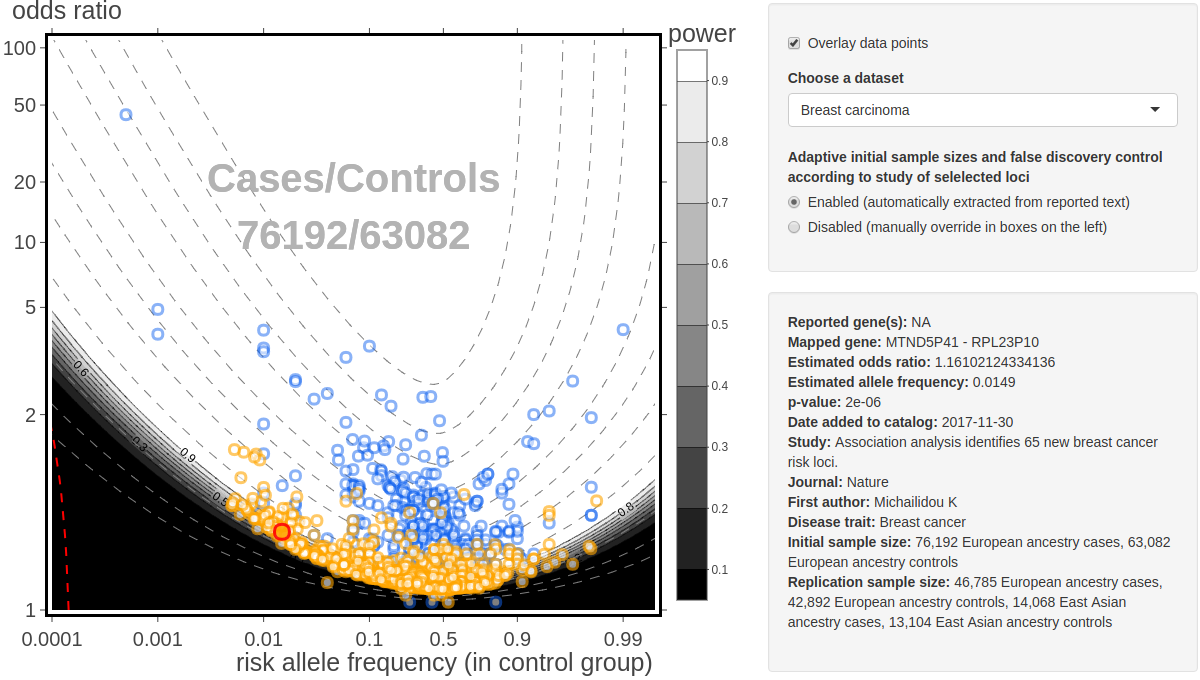
\includegraphics[width=0.48\textwidth]{Screenshot_GWAS_calculator6.eps}
% \vspace{-20pt}
% \caption{Snapshot of the application's user interface, displaying reported associations from breast cancer studies in the NHGRI-EBI GWAS Catalog (circles).
% % the reported odds ratios and risk allele frequencies in the control groups. 
% The findings are overlaid on the OR-RAF power diagram of association tests (greyscale heatmap).
% The initial sample sizes are dynamically adjusted, and automatically determined from texts of the article reporting the user selected loci (red circle). 
% Information of the selected loci and the articles are also dynamically displayed; findings reported in the same article are highlighted (orange circles).
% We provide finite sample corrections by marking the rare variant region(s) where asymptotic approximations do not apply (red dashed lines, lower-left).
% The majority of the published findings we surveyed exhibited a striking level of concordance with our theoretical predictions, with most associations congregating just inside the detectable region.
% }\label{fig:02}
% \vspace{-12pt}
% \end{figure}

\vspace{-5pt}
\subsection{Review and forensics of reported findings}

This unified treatment allows us to examine results from different studies in the same diagram, even when they do not employ the same model or statistical test.
This enables systematic reviews of reported findings for their statistical validity. 
In particular, a reported association predicted to have low power given the study's sample size -- lying in the dark regions of the OR-RAF diagram -- while not impossible, invites further scrutiny.%\footnote{It should be noted that a reported association predicted to have high power is not automatically accurate, as winner's curse induced by multiple testing may inflate the OR and RAF estimates \citep{Xiao09}.}

Studies where reported associations show misalignment with the predicted powered curves may be further investigated for potential problems.
% For example, the results of \citet{Dominguez-Cruz18} appear grossly misaligned when visualized using our method.
We reached out to one study where gross misalignment was identified \citep{Dominguez-Cruz18}. 
% The authors of the study confirmed with us that the RAF reported in the Catalog were based on all subjects in the study, as opposed to only the control group.
The authors of the study confirmed that this was the result of a problem in the data curation process of the GWAS Catalog (Dominguez-Cruz, personal communication).

The software provides options for users to load and overlay findings reported in the NHGRI-EBI GWAS Catalog, or upload data from other sources compliant with the Catalog's data format.

% In particular, for large samples, tests for zero slopes in logistic regressions should report approximately the same set of loci as Welch's t-tests for equal proportions on the same dataset, after the same family-wise error rate adjustments.
% The estimated odds ratios (in the case of logistic regression, estimate slopes exponentiated) and RAF's, when charted on the OR-RAF diagram, should also follow the same power limits.


\vspace{-5pt}
\subsection{Rare variants and finite sample corrections}

We address the quality of asymptotic approximations in our power analysis, as well as the applicability of single variant tests when rare genetic variants are present.
Specifically, we provide a lower bound on the variant counts needed to calibrate Fisher's exact test. 
If variant counts fall below the threshold, exact tests, and by extension, single-SNP-based association tests, cannot be correctly calibrated to have the desired type I error rate  without sacrificing all statistical power.
In such cases, the asymptotic approximations do not apply.
We mark this low-count, low-power region on the OR-RAF diagram.
See Supplement Sec. 2 for further details.

The software also provides options for users to specify the rare variant as 1) having less than a specified count, or 2) occurring in less than a percentage of all subjects in the study, as is customary in the literature.




